\documentclass[aspectratio=1610]{beamer}
\usepackage[utf8]{inputenc}
\usepackage[T1]{fontenc}
\usepackage[german]{babel}
\usepackage[useregional]{datetime2}
\usepackage[nameinlink]{cleveref}
\usepackage[section]{placeins}
\usepackage{xcolor}
\usepackage{graphicx}
\usepackage{csquotes}
\usepackage{amsmath} % for $\text{}$
\usepackage{enumitem}
\setlist{nosep}


\newcommand\urlpart[2]{$\underbrace{\text{\texttt{#1}}}{\text{#2}}$}
\raggedbottom
\crefname{figure}{Abb}{Abb}

\newcommand\producttitle{treff.}
\hypersetup{
	pdftitle={Entwurf: \producttitle},
	bookmarks=true,
}

% header & footer
\usepackage{scrlayer-scrpage}
%\lofoot{\today}
%\refoot{\today}
\pagestyle{scrheadings}

\title{
\includegraphics[width = 50mm]{images/logo_crop.png}}
\subtitle{\huge Entwurf}
\author{Lukas Dippon
	\and Jens Kienle
	\and Matthias Noll
	\and Fabian Röpke
	\and Tim Schmidt
	\and Simon Vögele}

\begin{document}

	\begin{frame}[plain]
	\maketitle
	\end{frame}

	\begin{frame}[plain]
        CLIENT (PLATZHALTER)
	\end{frame}

	\begin{frame}[plain]
        SERVER (PLATZHALTER)
	\end{frame}

	\begin{frame}[plain]
        API (PLATZHALTER)
	\end{frame}

    \begin{frame}[plain]
        \frametitle{Arbeitsweise}
        \begin{minipage}{0.5\textwidth}
            \only<1>{
                PLATZHALTER
                % treff.-Positionsicon, TeamSpeak-, Discord- und Telegram-Icon
            }
            \only<2>{
                PLATZHALTER
                % Screenshot vom Wekanboard
            }
            \only<3>{
                PLATZHALTER
                % Ordnerhierarchie (server,client,entwurf)?
            }
        	\only<4>{
        		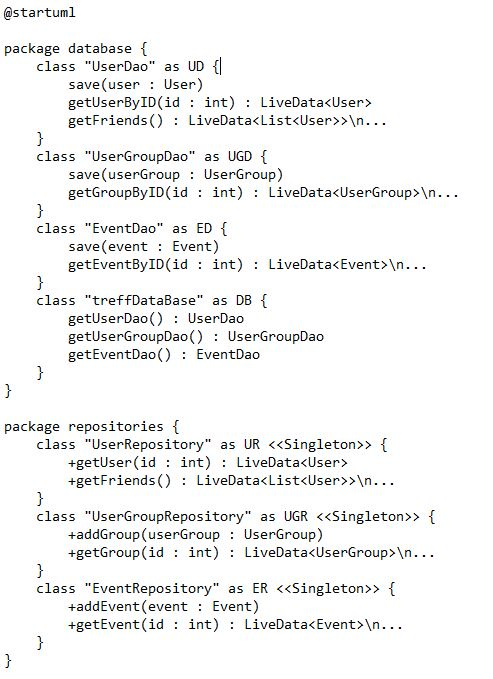
\includegraphics[height = \columnwidth]
        		{images/diagram.JPG}
        		% Diagrammcode, Lucidchart?
        	}
        \end{minipage}%
        \begin{minipage}{0.5\textwidth}
            \only<1>{
                \textbf{Kommunikation}
                \begin{itemize}
                    \setlength\itemsep{0.3em}
                    \item[--] Treffen mit allen Gruppenmitgliedern oder in
                        Teilgruppen
                    \item[--] Absprachen über die VoIP-Dienste TeamSpeak und
                        Discord und den Instant Messenger Telegram
                \end{itemize}
            }
            \only<2>{
                \textbf{Aufgabenverteilung und Notizen}
                \begin{itemize}
                    \setlength\itemsep{0.3em}
                    \item[--] Gemeinsame Notizen über Etherpad
                    \item[--] Festhaltung und Zuweisung von Teilaufgaben über
                        ein Kanbanboard	
                \end{itemize}
            }
            \only<3>{
                \textbf{Entwicklung der Struktur und Verfassung des Dokuments}
                \begin{itemize}
                    \setlength\itemsep{0.3em}
                    \item[--] Synchronisierung über Git
                    \item[--] Zwei separate Projekte für Klient und Server
                    \item[--] Entwurfsdokument geteilt in Inhalt (.tex) und
                        Formatierung (.sty)
                \end{itemize}
            }
        	\only<4>{
        		\textbf{Herausforderungen}
        		\begin{itemize}
        			\setlength\itemsep{0.3em}
        			\item[--] Unbekannte Dokumentform
        			\item[--] Differenzen zur Schulung, vieles \enquote{from 
        			Scratch}
        			\item[--] Übersichtliche Diagramme erstellen / 
        			automatisieren / synchronisieren
        			Formatierung
        		\end{itemize}
        	}
        \end{minipage}
    \end{frame}
\end{document}
